


\section{Разность разностей}
\subsection{Примеры}

\begin{frame}{Эффект реакции потребителей на экологическую катастрофу}
\begin{figure}
    \centering
    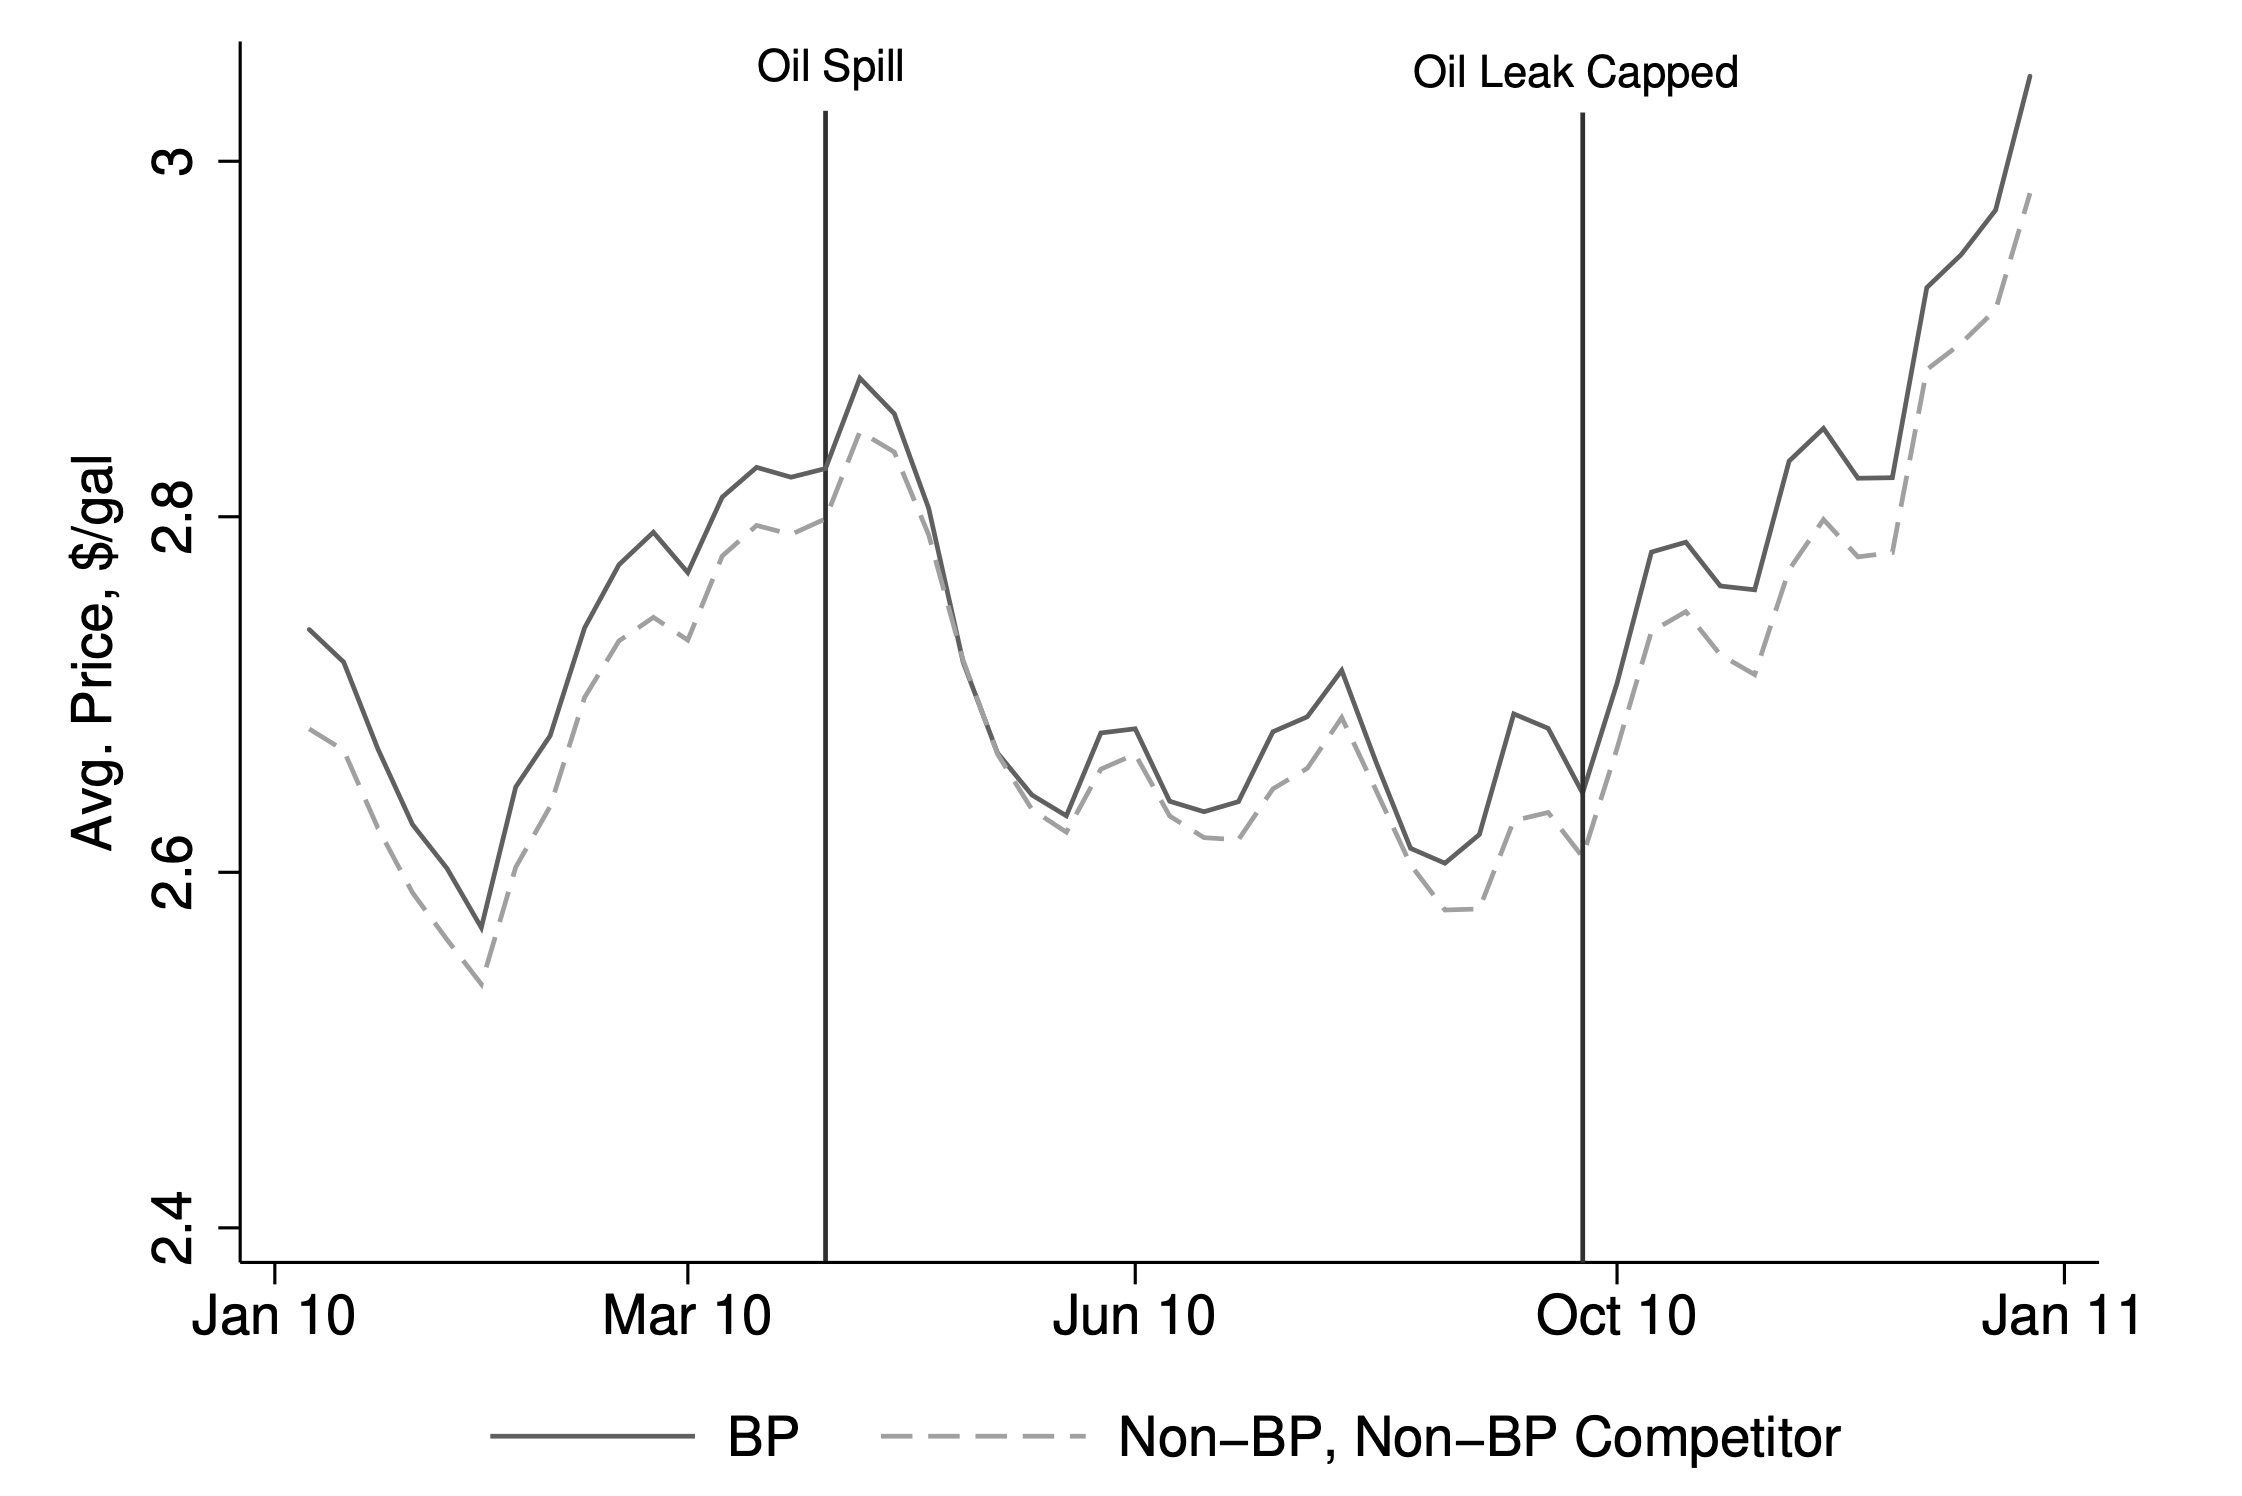
\includegraphics[width=\textwidth]{Images/oil.png}
    \label{fig:my_label}
\end{figure}
\end{frame}

\begin{frame}{Разница в доходе женщин с ребенком и мужчин с ребенком}
\begin{figure}
    \centering
    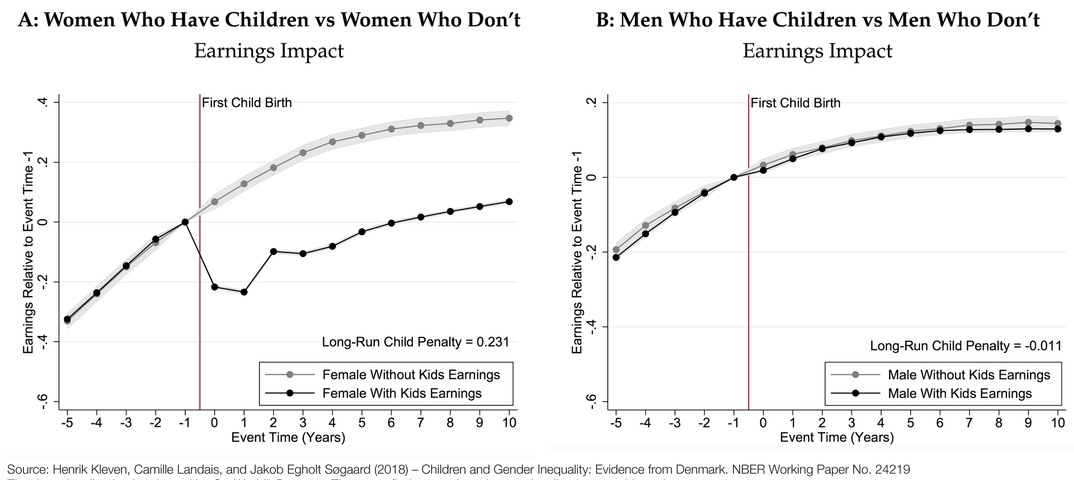
\includegraphics[width=\textwidth]{Images/gender.jpg}
    \label{fig:my_label}
\end{figure}
\end{frame}

\subsection{Предположения о данных}

\begin{frame}{Обозначения данных и предположения}
    \begin{itemize}
        \item Как обычно, потенциальные исходы: $(Y^0, Y^1, X)_{it}$
        \item Переменная воздействия: $T_{i}$
        \item Наблюдаемый $Y = Y^0 + T (t > 0) (Y^1 - Y^0)$
    \end{itemize}
    \pause
    Предпосылки идентификации:
    \begin{itemize}[<+->]
        \item Верно ли, что $(Y^1, Y^0, X) \perp T$ ?
        \item Верно ли, что $(Y^1, Y^0) \perp T | X$ ?
        \item Давайте хотя бы предположим $(\Delta Y^1, \Delta Y^0) \perp T | X$, где
        $\Delta Y^j = Y^j_{it} - (\bar Y^j)_{i, t < 0}$

    \end{itemize}
\end{frame}

\begin{frame}{Предпослыка идентификации}
    Общий тренд условно на X
    $$(\Delta Y^1, \Delta Y^0) \perp T | X$$
\end{frame}


\subsection{Примеры в линейной регрессии}


\begin{frame}{В линейной регрессии: примеры}
    Раньше мы всегда оценивали модель: $Y = \alpha + \tau T$
    
    Теперь мы будем оценивать: $Y_{it} - Y_i0 = \Delta Y_i = \alpha + \tau T_i$
    
    Альтернативно это можно записать как: 
    $$Y_{it} = \alpha_0 (t=0) + \alpha_1  (t=1) + \alpha_2 (t=2) + \tau_1 (t=1) T_{i} + \tau_2 (t=2) T_{i}$$
    
\end{frame}


% \begin{frame}{А как поступить, если у нас обычный эксперимент}
    
% \end{frame}

\begin{frame}{Placebo test}
\begin{figure}
    \centering
    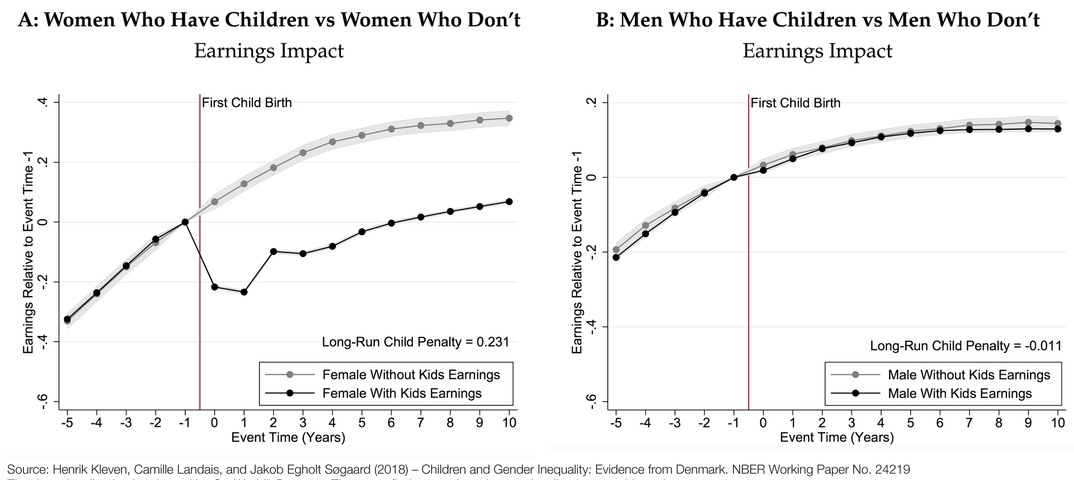
\includegraphics[width=\textwidth]{Images/gender.jpg}
    \label{fig:my_label}
\end{figure}
\end{frame}

\begin{frame}{Placebo test через регрессию}
\begin{align*}
    Y_{it} = & \alpha_{-2} (t=-2) + \alpha_{-1}  (t=-1) + \alpha_2 (t=0) + \\
    & \tau_{-2} (t=-2) T_{i} + \tau_{-1} (t=-1) T_{i}
\end{align*}*

Проверить, что $\tau_{-2} = \tau_{-1} = 0$

\end{frame}


% НУЖНА КРИТИКА -- ЧЕРЕЗ ОТСЕЧКУ МЕНЯЕТСЯ НЕ ТОЛЬКО
% здесь же про эту идею инструментов из worldbank
% anticipations
% ???


% НУЖЕН НОРМАЛЬНЫЙ ФОРМАЛИЗОВАННЫЙ ТЕСТ. А КРИТИКУ ТЕСТА С PARTIAL IDENTIFICATION потом
% https://blogs.worldbank.org/impactevaluations/revisiting-difference-differences-parallel-trends-assumption-part-ii-what-happens
% отдельно time series идея. в causal impact


% Если имеется определенная опытная группа, но отсутствует естественная контрольная группа, имеет смысл учитывать неопределенность, связанную с выбором контрольной группы. Такой подход предложен в Abadie, Diamond & Hainmueller (2007).
% Также существует подход описанный у Donald & Lang (2007). Постановка DL применима к общему случаю, когда число групп (контрольных и опытных) достаточно мало, и для каждой из них доступны довольно большие выборки. 
% Для большого числа групп можно использовать и временной интервал достаточно долгий. Тогда будет полезна общая модель, рассмотренная в BDM (2004) и Hansen (2007).
% Для оценки эффектов программ можно использовать оценку разности разностей через панельные данные на индивидуальном уровне Wooldridge (2002).
% Также можно применять полупараметрический или непараметрический подходы Athey & Imbens (2006).
